\let\negmedspace\undefined
\let\negthickspace\undefined
\documentclass[journal]{IEEEtran}
\usepackage[a5paper, margin=10mm, onecolumn]{geometry}
\usepackage{lmodern} % Ensure lmodern is loaded for pdflatex
\usepackage{tfrupee} % Include tfrupee package

\setlength{\headheight}{1cm} % Set the height of the header box
\setlength{\headsep}{0mm}     % Set the distance between the header box and the top of the text

\usepackage{gvv-book}
\usepackage{gvv}
\usepackage{cite}
\usepackage{amsmath,amssymb,amsfonts,amsthm}
\usepackage{algorithmic}
\usepackage{graphicx}
\usepackage{textcomp}
\usepackage{xcolor}
\usepackage{txfonts}
\usepackage{listings}
\usepackage{enumitem}
\usepackage{mathtools}
\usepackage{gensymb}
\usepackage{comment}
\usepackage[breaklinks=true]{hyperref}
\usepackage{tkz-euclide} 
\usepackage{listings}
\usepackage{gvv}                                        
\def\inputGnumericTable{}                       
\usepackage[latin1]{inputenc}                                
\usepackage{color}                                            
\usepackage{array}                                            
\usepackage{longtable}                                       
\usepackage{calc}                                             
\usepackage{multirow}                                         
\usepackage{hhline}                                           
\usepackage{ifthen}                                           
\usepackage{lscape}  
\usetikzlibrary{patterns}
\begin{document}
\bibliographystyle{IEEEtran}


\textbf{Question 4.4.22:} \\
 \textbf Find the equation of a plane which passes through the point $(3,2,0)$ and contains the line
\begin{align}
\frac{x-3}{1} \;=\; \frac{y-6}{5} \;=\; \frac{z-4}{4}.
\end{align}

\textbf{solution:}\\
\textbf{Finding the plane using column vectors.}

Let the normal be \(\vec{n}=(a,b,c)^T\). We use the form
\begin{align}
\vec{n}^T\vec{x}=1.
\end{align}

The plane passes through the point \(P=(3,2,0)\) and contains the line
\begin{align}
\frac{x-3}{1}=\frac{y-6}{5}=\frac{z-4}{4},
\end{align}
so take a point on the line \(A=(3,6,4)\) and the direction vector
\(\vec{v}=(1,5,4)\).

The conditions are
\begin{align}
\vec{n}^T\vec{P} = 1
\end{align}
\begin{align}
\vec{n}^T \vec{A} = 1
\end{align}
\begin{align}
\vec{n}^T \vec{v} = 0.
\end{align}

Put these three column vectors together into a matrix (columns are the given points/vectors):
\begin{align}
\vec{M}=\begin{myvec}{
3 & 3 & 1\\[4pt]
2 & 6 & 5\\[4pt]
0 & 4 & 4}
\end{myvec}
\qquad\text{(columns are }\vec{P},\;\vec{A},\;\vec{v}\text{).}
\end{align}

Then the three scalar conditions above read compactly as
\begin{align}
\vec{n}^T\vec{M} = \begin{myvec}{1 & 1 & 0}\end{myvec}.
\end{align}
Transposing both sides gives a standard linear system for \(\vec{n}\):
\begin{align}
\vec{M}^T \vec{n} = \begin{myvec}{1\\[4pt]1\\[4pt]0}\end{myvec}.
\end{align}

Write this out:
\begin{align}
\begin{myvec}{
3 & 2 & 0\\[4pt]
3 & 6 & 4\\[4pt]
1 & 5 & 4
}\end{myvec}
\begin{myvec}{a\\[4pt]b\\[4pt]c}\end{myvec}
=
\begin{myvec}{1\\[4pt]1\\[4pt]0}\end{myvec}.
\end{align}
\begin{align}
\vec{n}
=
\begin{myvec}{1\\-1\\1}\end{myvec}.
\end{align}

Thus a convenient normal vector is \(\vec{n}=(1,-1,1)^T\), and the plane equation in the requested form is
\begin{align}
\begin{myvec}{1\\-1\\1}^T\end{myvec}\vec{x}=1
\end{align}
\begin{figure}[h!]
    \centering
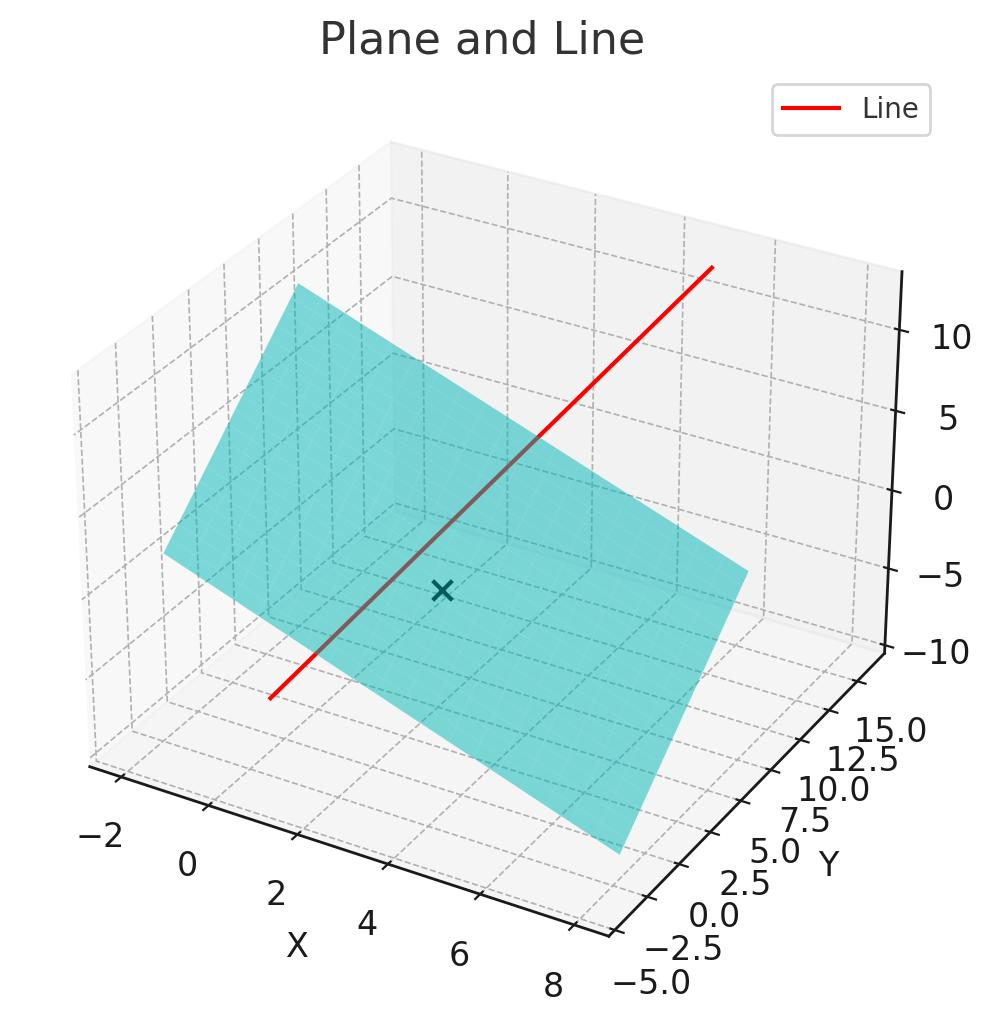
\includegraphics[width=0.5\linewidth]{beamer/figs/mat7.jpeg}
    \caption{}
    \label{fig:placeholder}
\end{figure}
\end{document}
